%
\section{提案手法}
\label{ch:methodology}
%
\subsection{モデル概観}
この章では,提案モデルがもつ複合特徴量抽出器とニュース分類器について紹介する.
その後にこの2要素を統合して転移学習が可能な表現を学習する方法について説明する.
% 最後に,詳細なアルゴリズムフローを付加する. 
今回提案したモデルは,以下の図\ref{fig:model}の通りである.

提案モデルの目的は,画像と文章で発信された情報に対して,
正しいニュースか・フェイクニュースか・ジョークニュースかを分類するために,
必要な特徴表現を学習することであった.
提案モデルは複合特徴量抽出器とニュース分類器の大きく2部分に分けることができた.
まず複合特徴量抽出器は,今回扱う情報が文章と画像を含むため,
各メディアに対して特徴化する抽出器があった.
その後それぞれの特徴を1つに連結し,複合特徴を形成した.
複合特徴はニュース分類器に送られ,最終的には3カテゴリのどれに該当するかが判断された.
% 
\begin{figure*}[tb]
    \centering
    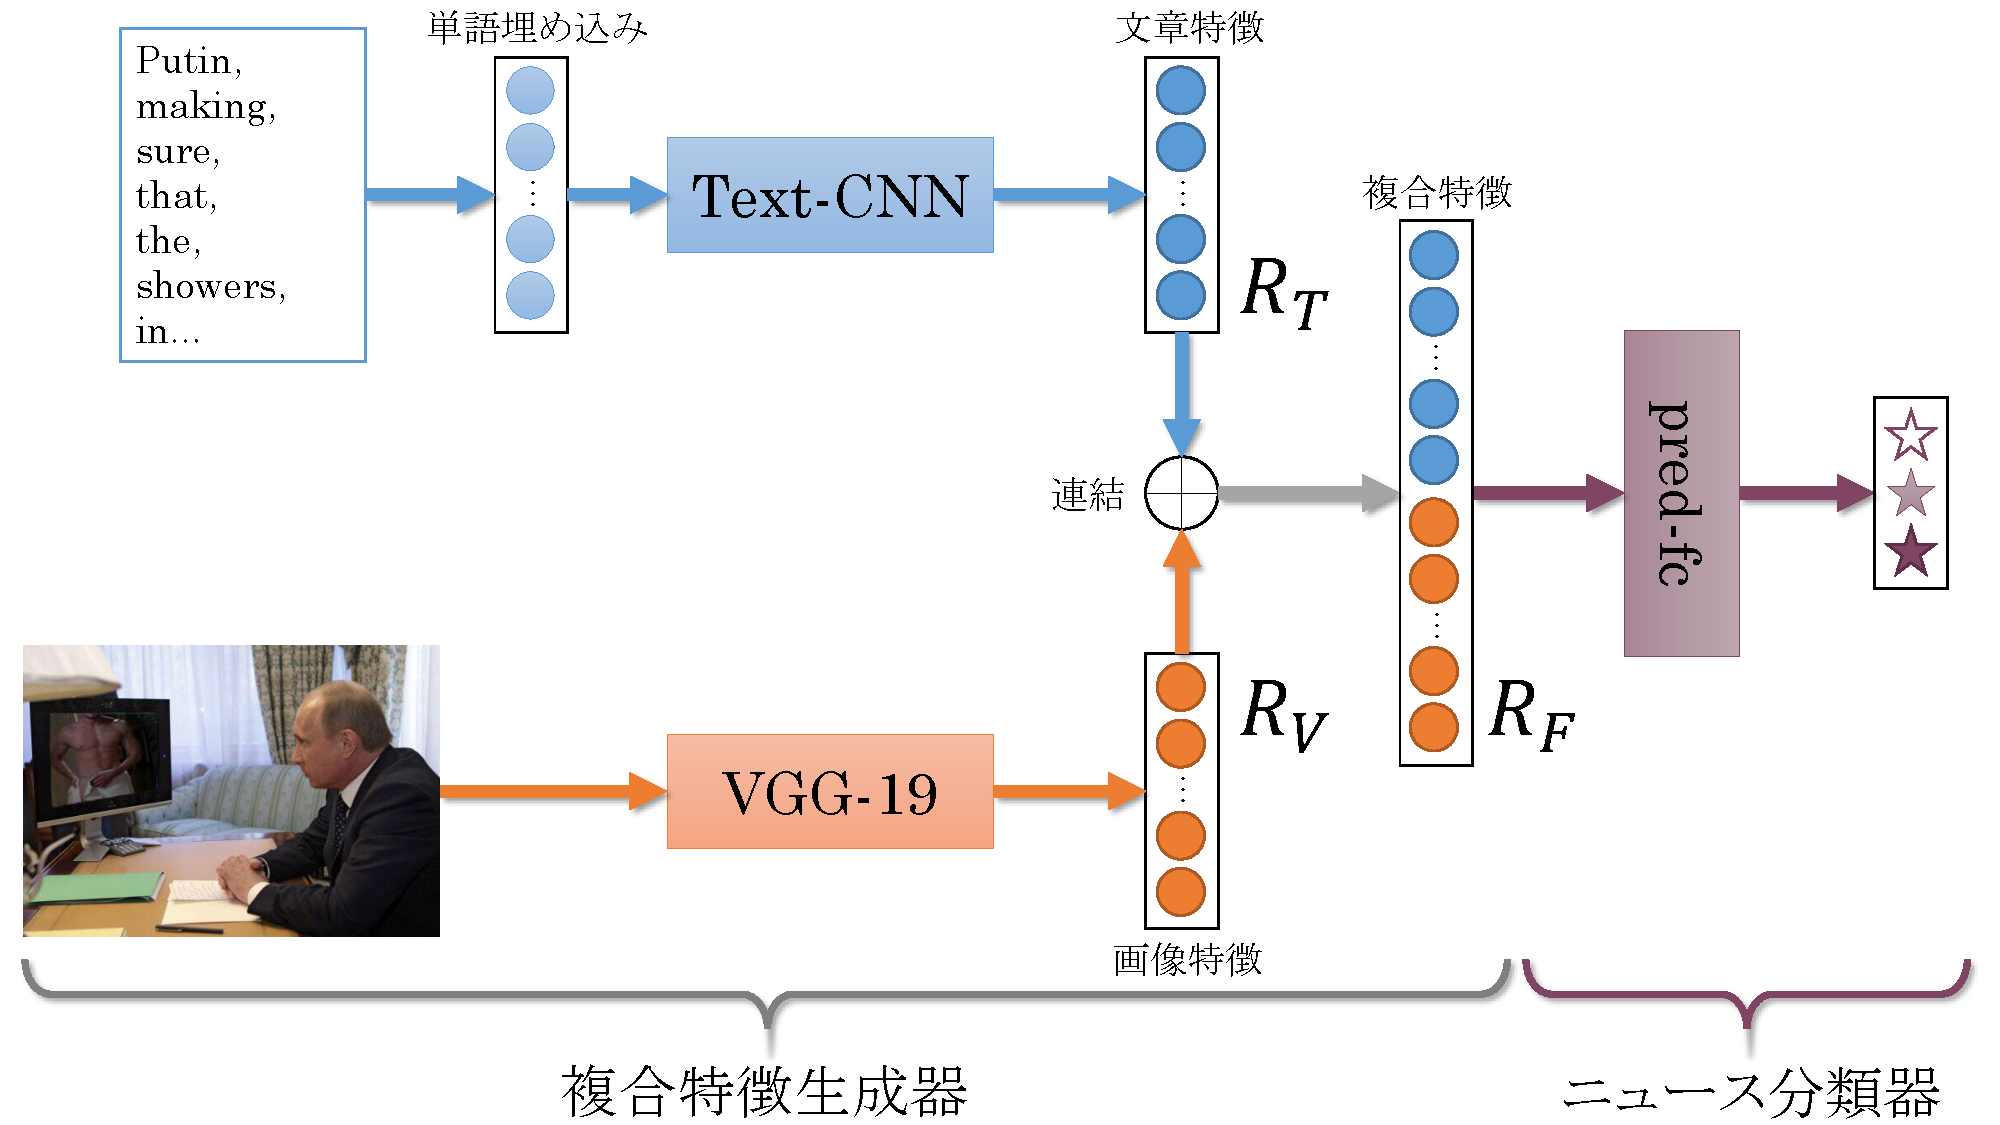
\includegraphics[width=0.8\linewidth]{images/methodology.pdf}
    \caption{提案モデル図.青: 文章特徴量抽出器,橙: 画像特徴抽出器,紫: ニュース分類器.}
    \label{fig:model}
\end{figure*}
%
\subsection{複合特徴抽出器}
%
\subsubsection{文章特徴} \label{subsec:text}
文章特徴は,入力に英語の投稿をスペース毎に分割した英単語の連続リストをもった.
まずは単語を単語埋め込みでベクトル化した.
その後単語の羅列から分類に有効な情報を得るために,文章特徴を抽出する核としてCNN
(convolutional neural networks: 畳み込みニューラルネットワーク)を採用した.
CNNはコンピュータビジョンやテキスト分類などの多くの分野で効果的であることが示されていた
\cite{collobert2011natural,KalchbrennerACL2014}.
図\ref{fig:model}の通り,提案手法ではCNNの発展形であるテキストCNN(Text-CNN)\cite{DBLP:journals/corr/Kim14f}を採用した.
テキストCNNの構造は図\ref{fig:text-cnn}の通りである.
複数のウィンドウで畳み込むことで,様々な角度から特徴を抽出することを実現した.
\begin{figure}[H]
    \centering
    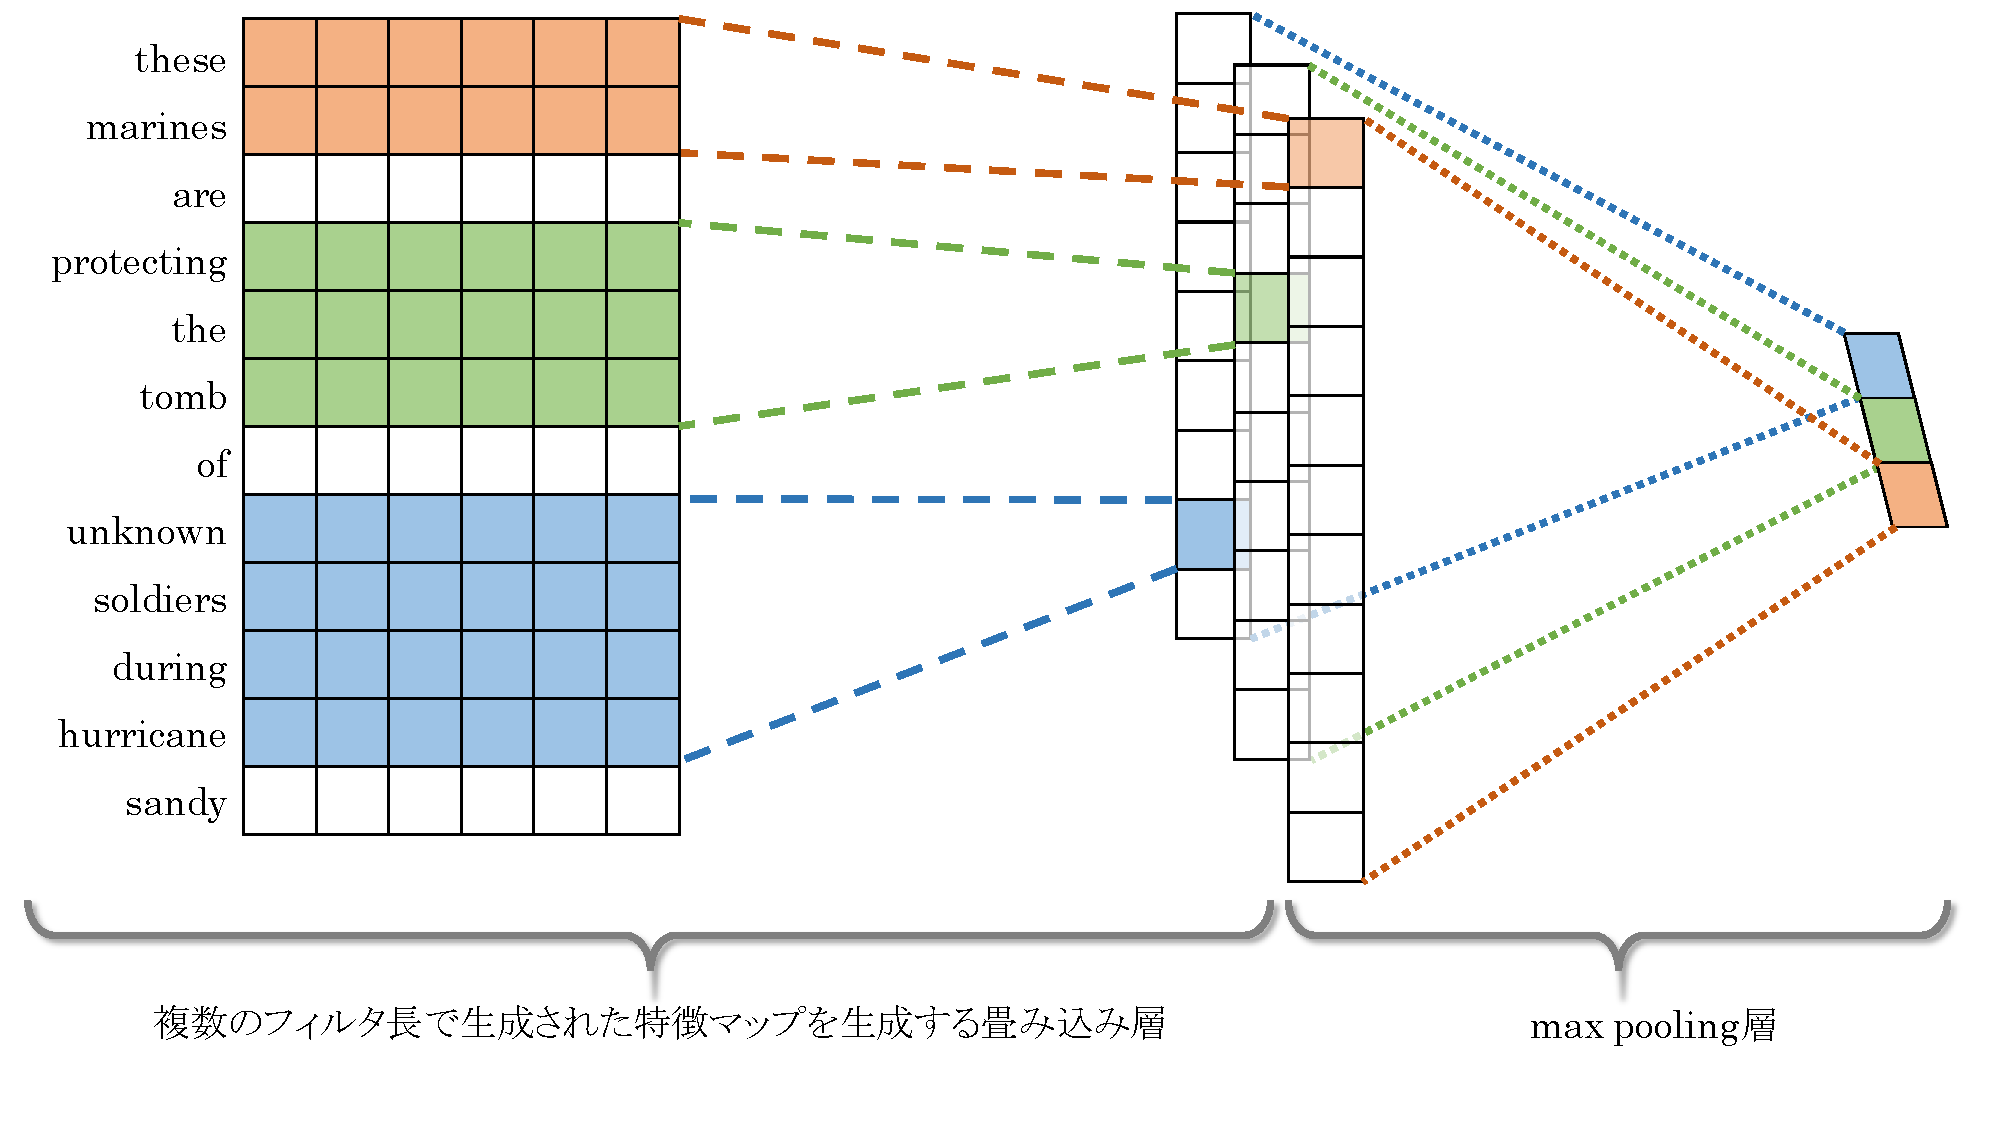
\includegraphics[width=\linewidth]{images/text-cnn.pdf}
    \caption{テキストCNNの図.Wangらの研究\cite{Wang:2018:EEA:3219819.3219903}を参考に作成.}
    \label{fig:text-cnn}
\end{figure}

具体的な手法では,EANNが採用したテキストCNNと同じ流れを汲み\cite{Wang:2018:EEA:3219819.3219903},
最終の全結合層の隠れ層に独自にdropoutを採用した形をとった.
今回使用した文章特徴抽出器の理論式を以下に引用する.

投稿の$i$番目の単語を$k$次元の単語埋め込みに変換する際に抽出された単語埋め込みベクトルを$T_i \in \mathbb{R}^k$とする.
このとき,$n$単語から抽出された投稿は以下の式\ref{eq:concat_emb}で表現ができる.
\begin{equation}
    \label{eq:concat_emb}
    T_{1:n} = T_1 \oplus T_2 \oplus \ldots \oplus T_n,
\end{equation}
$\oplus$はベクトルを連結(concatenation)することを意味する記号である.
ここで単語埋め込み化された投稿は,畳み込み層へ送られる.
畳み込み層では$h$単語分のウィンドウサイズがある.
これは単語埋め込み化された投稿から連続して取り出す単語埋め込みベクトルの数を意味する.
$i$番目を基準に$h$単語分取り出された場合,フィルタ時の処理は以下の式\ref{eq:filter}の通りである.
\begin{equation}
    \label{eq:filter}
    t_i = \sigma(W_c \cdot T_{i:i+h-1}).
\end{equation}
この$\sigma(\cdot)$は活性化関数の1つであるReLU(ランプ関数)を表し,$W_c$はフィルタの重みを意味する.
式\ref{eq:filter}が投稿内で適用されると,式\ref{eq:feature}の通り1つの発言に対し1つの特徴ベクトルが得られる.
\begin{equation}
    \label{eq:feature}
    t = [t_1, t_2, \ldots, t_{n-h+1}].
\end{equation}
この$t$ベクトルに対して最も重要な特徴を得るために,ベクトル内で最大値の要素のみを取り出すmax-poolingが行われる.

これで1つのウィンドウサイズから1つの特徴が得られるが,
多くの粒度の特徴を得るために当手法では複数のウィンドウサイズから複数の値を取得している.
特定のウィンドウサイズに着目すると,$n_h$分異なるフィルタが存在することになる.
もし使用可能なウィンドウサイズが$c$存在する場合,全体で$c \cdot n_h$だけフィルタが存在することとなる.
投稿から各ウィンドウサイズでmax-poolingまでされた文章特徴は$R_{T_c} \in \mathbb{R}^{c \cdot n_h}$と表現できる.

max-poolingを終えた文章特徴は全結合層に渡され,
最終的に式\ref{eq:image-fc}によって
画像特徴抽出器が出力する特徴ベクトルの次元($p$とする)に合わせたテキスト特徴$R_T \in \mathbb{R}^p$となる.
\begin{equation}
    \label{eq:image-fc}
    R_T = \sigma(W_{tf} \cdot R_{t_c}),
\end{equation}
ここで$W_{tf}$は全結合層における重みを意味する.なお,この全結合層では隠れ層にdropoutを当研究では採用した.
dropoutはHintonらによって提案された手法\cite{JMLR:v15:srivastava14a}で,
学習時に指定された確率で無作為に$W_{tf}$内の要素を無効化(0に)してモデルの自由度を制限する.
これにより,モデルが訓練データセットに特化しすぎて汎用性が失われる過学習に繋がりにくくなる利点が報告されていたため,採用した.
%
\subsubsection{画像特徴}
画像から効率的に特徴を抽出するために,当研究では事前学習済みのVGG19\cite{DBLP:journals/corr/SimonyanZ14a}を起用した.
VGG19は畳み込み16層と全結合層3層から形成され,最終的には1000次元の特徴ベクトルが出力される.
当研究では最終の全結合層のみ改変し,文章特徴のベクトル次元数と同じ数の次元をもつベクトルを出力するようにした.
また改変した最終全結合層以外は,過学習を防ぐために事前学習の状態を維持することにした.

第\ref{subsec:text}節で記したように,最終的な特徴ベクトルの次元数は$p$とする.
VGG19では畳み込み16層で$7 \times 7 \times 512$の行列となり,
その後2層の全結合層によって$1 \times 1 \times 4096$に整形され,
最終第三全結合層(fc19)によって$1 \times 1 \times 1000$の画像特徴ベクトルを出力する.
Wangらの研究\cite{Wang:2018:EEA:3219819.3219903}ではVGGのfc19の出力を$p$に整形していたが,
当研究では直接fc19を改変して$1 \times 1 \times p$の画像特徴ベクトルを出力するようにした.
この改変したfc19によって算出される画像特徴$R_V \in \mathbb{R}^p$は以下の式\ref{eq:fc19}の通りである.
\begin{equation}
    \label{eq:fc19}
    R_V = \sigma(W_{vf} \cdot R_{V_{\rm VGGfc18}}),
\end{equation}
$R_{V_{\rm VGGfc18}}$はVGG19の第18層である全結合層が出力した$1 \times 1 \times 4096$ベクトルである.

こうして文章特徴・画像特徴が抽出され,最終的には2つの特徴ベクトルを1つに連結したものが複合特徴である.
理論式で表記すると,文章特徴$R_T$と画像特徴$R_V$が1つに結合されるため,
複合特徴$R_F$は以下の式\ref{eq:concat_feature}によって表現できる.
\begin{equation}
    \label{eq:concat_feature}
    R_F = R_T \oplus R_V \in \mathbb{R}^{2p}.
\end{equation}
以降においては,複合特徴抽出器全体を表現するときは$G_f(M; \theta_f)$と表現することにする.
$M$は複合特徴抽出器へ入力される投稿,$\theta_f$は学習対象となるパラメータを意味する.
%
\subsection{ニュース分類器}
%
複合特徴はニュース分類器(図\ref{fig:model}内`pred-fc'が該当)にて正しいニュース・フェイクニュース・ジョークニュースとして分類された.
具体的には隠れ層を含む全結合層とsoftmaxから形成され,最終的な分類が行われた.
この部分の理論式は以下の通りである.

入力となる複合特徴は$R_F$であるとき,ニュース分類器は$G_f(\cdot; \theta_d)$と表現することにする.
ここで$\theta_d$はニュース分類器内で学習対象となるパラメータを示す.
投稿全体に対して$i$番目の投稿を$m_i$とするとき,
$m_i$がフェイクニュースもしくはジョークニュースである確率は以下の式によって算出される.
\begin{equation}
    \label{eq:news_classify}
    P_\theta(m_i) = G_d(G_f(M; \theta_f); \theta_d).
\end{equation}
モデルの目的は自動で正確に正しいニュース・フェイクニュース・ジョークニュースを分類することである.
そのため正解ラベルとして$Y_d$を使用して,以下の式によってクロスエントロピー誤差を損失として算出する.
\begin{multline}
    \label{eq:cross_entropy}
    L_d(\theta_f, \theta_d) =\\
    -\mathbb{E}{(m,y)~(M, Y_d)}[y\log P_\theta(m) + (1-y)\log (1-P_\theta(m))].
\end{multline}

最後に,当研究がベースとしたWangらの研究では確率的勾配降下法(SGD: Stochastic Gradient Descent)
によってパラメータを更新していたが,
当研究では2015年にDiederik P. Kingmaらが提唱したAdamという手法\cite{DBLP:journals/corr/KingmaB14}
を用いてパラメータを更新することにした.
%

